\chapter[Teoretická část studentské práce]{Teoretická část studentské\\ práce}

\section{Principy pořizování rentgenových snímků}
\label{sec:principy}
Pořizování rentgenových snímků je prováděno pomocí zdroje \zk záření, rentgenovaného objektu a detektoru rentgenového záření. Rentgenové záření jsou elektromagnetické vlny s vlnovou délkou od \SI{10}{\nano\meter} do \SI{1}{\pico\meter} jejichž enerigie se nejčastěji pohybuje od \SI{1}{\kilo\eV} do \SI{200}{\kilo\eV}. \cite{AstroNuklFyzika-JadRadFyzika}

Jak již bylo zmíněno výše, scéna pro pořizování rentgenových snímků (\cref{fig:xray-scene}) se skládá ze zdroje rentgenového záření, rentgenovaného objektu a detektoru rentgenového záření. Zdroj rentgenového záření ozařuje elektromagnetickým vlněním o vlnové délce \SI{5}{\pico\meter} až \SI{50}{\pico\meter} rentgenovaný objekt. V závislosti na tloušťce a absorpčních vlastnostech objektu se část záření absorbuje a zbylá část záření dopadá na detektor rentgenového záření. Výstupem detektoru je poté obraz ve stupních šedi. \cite[kap.~3.2]{AstroNuklFyzika-JadRadMetody}

\begin{figure}[bh]
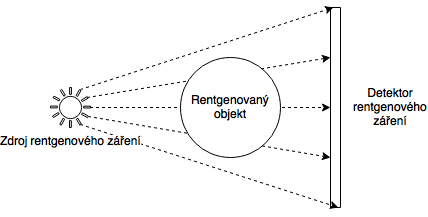
\includegraphics[width=\textwidth]{xray-scene}
\caption{Scéna pro pořizování rentgenových snímků.}
\label{fig:x-ray-scene}
\centering
\end{figure}

\subsection{Vznik rentgenového záření}
\label{sec:vznik-rentgenoveho-zareni}
Elektromagnetické záření, kterému se říká rentgenové záření vzniká buď při přechodu elektronů mezi vnitřními vrstvami těžších atomů -- charakteristické X-záření, nebo při dopadu a prudkém zabrzdění elektronů -- brzdné záření. \cite{AstroNuklFyzika-JadRadFyzika}

\subsubsection{Brzdné záření}
V případě, že se akcelerovaný elektron přiblíží k jádru atomu silné Coulombovy síly mezi jádrem atomu a letícím elektronem způsobí silné zbrzdění elektronu a změnu jeho trajektorie. Během zbrzdění rychle letícího elektronu  je jeho kinetická energie přeměňována na brzdné záření. \cite[str.~89]{Diagnostic-Radiology-Physics} Tento proces popisuje \cref{fig:bremsstrahlung-xray}.

\begin{figure}[bh]
\centering
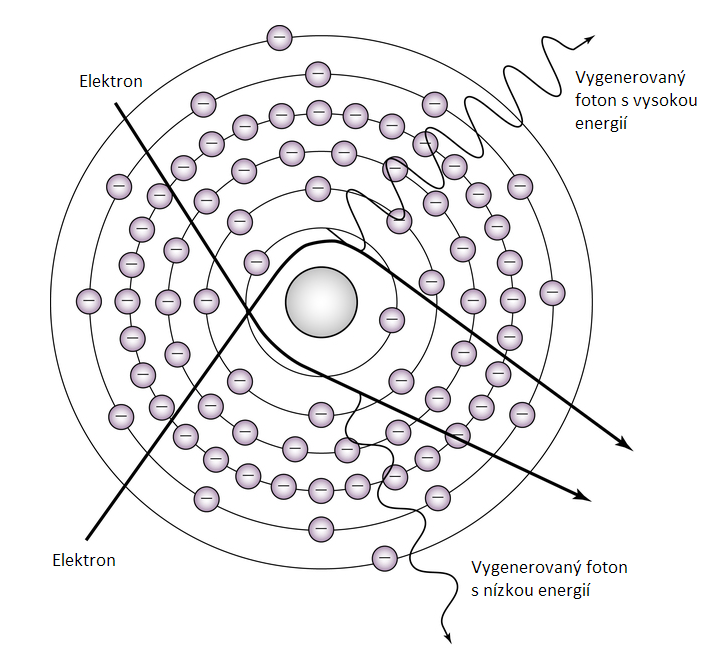
\includegraphics[width=0.75\textwidth]{bremsstrahlung-xray}
\caption{Vznik brzdného záření při interakci rychle se pohybujícího elektronu s atomem wolframu. \cite{the-xray-beam}}
\label{fig:bremsstrahlung-xray}
\end{figure}

Ideální spektrum brzdného záření lze popsat pomocí zjednodušeného modelu, který neuvažuje kvantovou mechaniku. Zjednodušený model uvažuje proud elektronů přibližující se k atomu. Uvážíme-li pole v okolí jádra atomu rozdělené na několik kruhových vrstev dle působících brzdných sil, generované brzdné záření brzděním proudu elektronů má spektrum, které odpovídá plochám těchto vrstev. Čím blíže je vrstva pole k jádru atomu, tím větší brzdnou sílou působí na letící elektron a tím větší je energie vygenerovaného fotonu. Zároveň čím je vrstva pole vzdálenější od jádra atomu, tím větší má plochu a tím více fotonů je schopna vygenerovat. Fotony generované ve vzdálenějších vrstvách mají nižší energii vzhledem k nižším brzdným silám působících na přibližující se elektrony. \cite[kap.~THE~X-RAY TUBE]{The-Physical-Principles-of-Medical-Imaging}

Ideální spektrum brzdného záření zjednodušeného modelu ukazuje \cref{fig:bremsstrahlung-xray-char}. Ze spektra je zřetelné, že největší energii, která se blíží kinetické energii elektronů má jen zlomek z celkového počtu generovaných fotonů (fotony generované elektrony, které byly zabrzděny ve vrstvě nejblíže jádru).

\begin{figure}[bh]
\centering
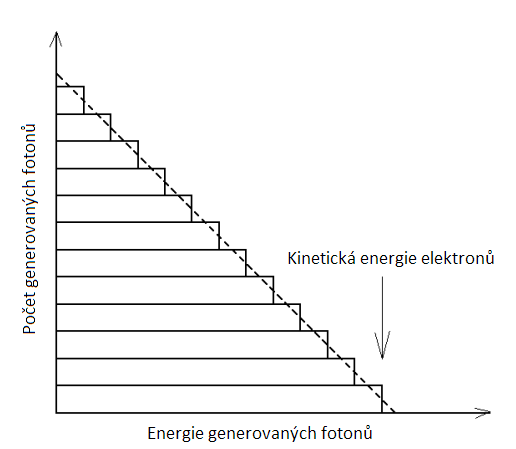
\includegraphics[width=0.75\textwidth]{bremsstrahlung-xray-char}
\caption{Ideální spektrum brzdného záření. \cite[str.~90]{Diagnostic-Radiology-Physics}}
\label{fig:bremsstrahlung-xray-char}
\end{figure}

\subsubsection{Charakteristické záření}
Charakteristické záření vzniká při přechodu atomového elektronu z vyšší vrstvy do nižší. Při přechodu elektron ztrácí energii, která je emitovaná jako foton charakteristického záření. Energie emitovaného fotonu odpovídá rozdílu energií vrstev mezi kterými elektron přechází. Spektrum charakteristického záření je monochromatické a odvíjí se od druhu atomu. Proces vzniku charakteristického záření popisuje \cref{fig:characteristic-xray}. \cite[str.~91]{Diagnostic-Radiology-Physics}

\begin{figure}[h]
\centering
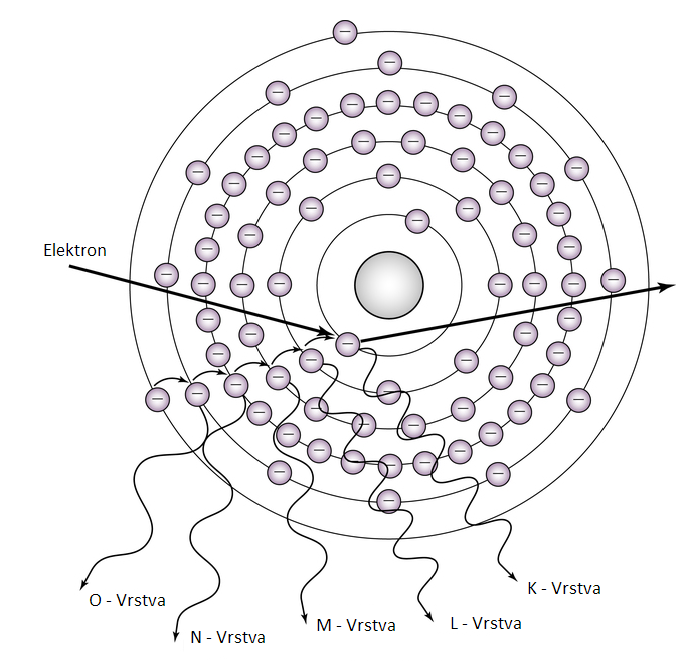
\includegraphics[width=0.75\textwidth]{characteristic-xray}
\caption{Vznik charakteristického záření v atomu wolframu při vyražení elektronu z K-Vrstvy elektronem s kinetickou energií vyšší, než vazební energie vyraženého elektronu. \cite{the-xray-beam}}
\label{fig:characteristic-xray}
\end{figure}

\subsection{Rentgenka}
Zdrojem rentgenového záření při pořizování rentgenových snímků je nejčastěji speciální vakuová elektronka (\cref{fig:xray-tube}), které je často nazývána jako rentgenka, rentgenová lampa či rentgenová trubice. \cite{AstroNuklFyzika-JadRadMetody} Rentgenku si lze představit, jako zařízení, které převádí energii elektronů na elektromagnetické záření s odpovídající energií. Expozice a spektrum záření může být řízena nastavením parametrů rentgenky jako jsou napětí (\SI{}{\kV}), proud (\SI{}{\mA}) a doba expozice (\SI{}{\s}). \cite[str.~93]{Diagnostic-Radiology-Physics}

\subsubsection{Principy fungování rentgenky}
Energie, která je přeměňována v rentgence na rentgenové záření a teplo je do rentgenky přiváděna proudem elektronů s potenciální energií odpovídající napětí na vysokonapěťovém zdroji (\SI{1}{\kV} odpovídá \SI{1}{\k\eV}). 
Během průchodu elektronu rentgenkou dochází k přeměně jeho potenciální energie na energii kinetickou, která je následně přeměněna na elektromagnetické záření a teplo. 

Kinetická energie elektronu při dopadu na anodu odpovídá napětí na vysokonapěťovám zdroji, tedy původní potenciální energii. Kinetická energie je přeměňována zbrzdění atomů při dopadu na anodu  při interakci s atomy materiálu na brzdné a charakteristické rentgenové záření. \cite[kap.~ELECTRON ENERGY]{The-Physical-Principles-of-Medical-Imaging}
Proud elektronu je emitován při žhavení katody se záporním napětí. Množství emitovaných elektronů může být řízeno změnou proudu žhavení, tedy změnou teploty žhaveného vlákna. \cite[str.~93]{Diagnostic-Radiology-Physics} 

\paragraph{Spektrum rentgenového záření rentgenky}
popisuje \cref{fig:xray-spectre}. Při dopadu elektronů na anodu vznikají dva typy rentgenového záření--brzdné a charakteristické, jejichž obecné principy byly popsány v kapitole \ref{sec:vznik-rentgenoveho-zareni}. Obrázek ukazuje celkem tři charakteristiky záření při napětí na elektrodách \SI{90}{\kV}:
\begin{enumerate}[label=(\alph*)]
\item Ideální spektrum brzdného brzdného záření--spektrum, které již bylo popsáno v obrázku \ref{fig:bremsstrahlung-xray-char}.
\item Generované spektrum--reálné spektrum skládající se z brzdného a charakteristického záření.
\item Filtrované spektrum--spektrum s útlumem dopovídajícím \SI{2.5}{\mm}Al.
\end{enumerate}

\begin{figure}[hb]
\centering
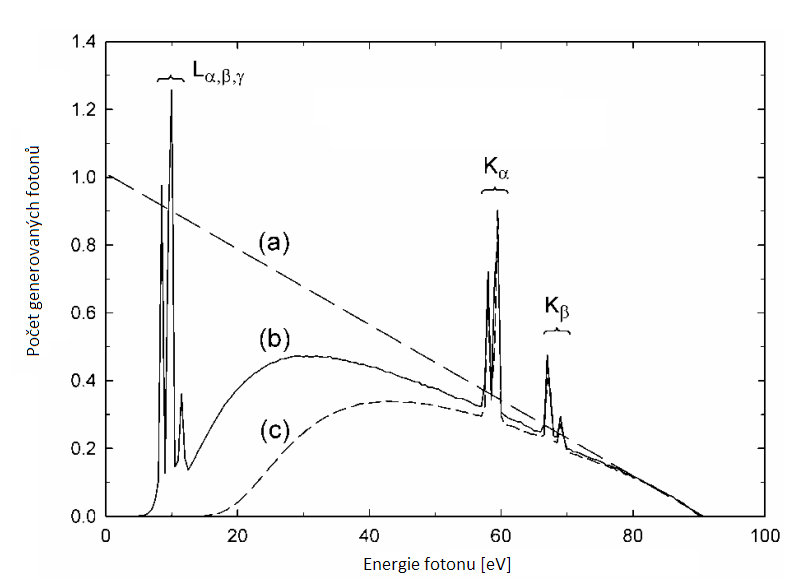
\includegraphics[width=\textwidth]{xray-spectre}
\caption{Rentgenka se zdroji proudu a napětí. \cite[str. 93]{Diagnostic-Radiology-Physics}}
\label{fig:xray-spectre}
\end{figure}

\subsubsection{Konstrukce rentgenky}
Z důvodu tepelného ohřevu anody po dopadu zrychlených elektronů a vysokého napětí na elektrodách musí být rentgenky oproti běžným elektronkám robustní konstrukce. Chlazení samotné anody je zajištěno její velikostí a také rotací  nebo aktivním chlazením. Rentgenky lze rozdělit kategorií podle způsobu využití a konstrukce \cite[kap. 3.2]{AstroNuklFyzika-JadRadMetody}:
\begin{itemize}
\item Rentgenky pro průmyslové ozařování a radioterapeutické použití - rentgenky s pevnou anodou, kde je chlazení zajištěno průtokem chladícího média. U toho typu rentgenek je častým požadavkem vysoká energie a intenzita záření. Naopak zde není potřebné zaměřování elektronů do téměř bodového ohniska. 
\item Rentgenky pro rentgenovou diagnostiku - rentgenky se soustředěním elektronů do ohniska. U tohoto typu rentgenek se využívá rotující anody proti nadměrnému přehřívání anody v místě ohniska.
\item Speciální rentgenky - rentgenky rozšířené o třetí elektrodu (drátěnou mřížku umístěnou mezi katodou a anodou v těsné blízkosti katody) sloužící k řízení proudu protékajícího anodou. Proud je řízen napětím, které je přivedeno na drátěnou mřížku.
\end{itemize}

Generované záření ještě před tím, než opustí rentgenku musí projít skrz různé materiály, které záření filtrují. Těmito materiály mohou být například samotná anoda, materiál trubice rentgenky, chladící medium apod. Úbytek záření při průchodu těmito materiály se uvádí jako útlum ekvivalentní k \SI{1}{\mm}Al--jednomu milimetru hliníku. Typická hodnota útlumu u běžných rentgenek bývá od \SI{0.5}{\mm}Al do \SI{1}{\mm}Al. 

\begin{figure}[hb]
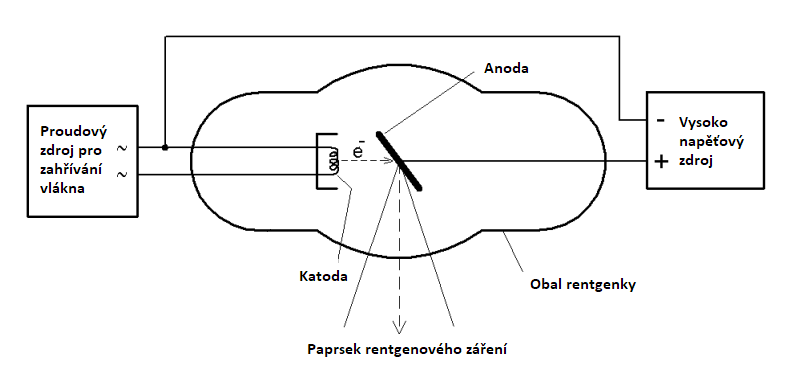
\includegraphics[width=\textwidth]{xray-tube}
\caption{Rentgenka se zdroji proudu a napětí. \cite[str. 93]{Diagnostic-Radiology-Physics}}
\label{fig:xray-tube}
\centering
\end{figure}

\paragraph{Anoda}
je součást rentgenky, kde je generováno rentgenové záření. Anoda bývá tvořena relativně velikým kusem železného materiálu, na který je přivedeno kladné napětí vysokonapěťového zdroje. Anoda jako taková plní v rentgence dvě funkce:
\begin{itemize}
\item Převod elektrické energie na rentgenové záření.
\item Odvod tepla, které vzniká během procesu generování rentgenového záření.
\end{itemize}
Jako vhodný materiál anody lze považovat materiál, který dokáže co největší podíl elektrické energie převést na záření, čili materiál, který má vysokou efektivitu převodu (jak již bylo zmíněno přebytečná energie je přeměňována na teplo). Efektivita převodu elektrické energie na záření závisí na atomovému číslu materiálu anody (Z) a kinetické energii dopadajícího elektronu na katodu.\cite{The-Physical-Principles-of-Medical-Imaging}

Nejvíce rentgenek využívá jako materiál anody wolfram s atomovým číslem 74. Wolfram je vhodný díky vysokému atomovému číslu a vysokému bodu tání. V některých případech je využíváno slitiny wolframu a rhenia, která je však využívána pouze jako povrchový materiál. Zbylá část anody anody poté bývá vyrobena z relativně lehkého materiálu, který má dobré tepelné vlastnosti. Těmito materiály mohou být například molybden nebo grafit. Výjimkou jsou anody rentgenek pro mamografii, kdy je využíváno molybdenu jako materiálu pro povrch anody.\cite{The-Physical-Principles-of-Medical-Imaging}

Anody lze dělit v závislosti na výkonu rentgenky (\cref{fig:anodes}). Pro aplikace, kdy není potřebná vysoká energie rentgenového záření je využíváno statických anod. Tato anoda se skládá z wolframu, který je usazen v měděném bloku, který slouží k odvádění tepla. Tento typ anod se využívá například dentistických nebo přenosných rentgenkách. Druhým typem anod jsou rotační anody. Anoda je připojená k rotoru asynchronního motoru, který je umístěn přímo ve vakuové trubici rentgenky. Vinutí statoru je naopak umístěno vně rentgenkové trubice. Samotná anoda má kruhový tvar v podobě terče se skosenými hranami na okrajích. Paprsek elektronů poté dopadá na zkosenou hranu, která je otáčena rotorem, tudíž je anoda tepelně namáhána rovnoměrně podél celého obvodu, což umožňuje generovat záření s vyšší energií. \cite{Diagnostic-Radiology-Physics}

\begin{figure}[hb]
\centering
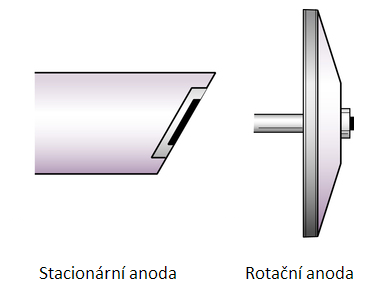
\includegraphics{anodes}
\caption{Rotační a stacionární anoda. \cite{the-xray-beam}}
\label{fig:anodes}
\end{figure}


\paragraph{Katoda}
je druhou elektrodou rentgenky, která má za úkol generování paprsku elektronů pomocí žhavícího vlákna (\cref{fig:cathode}). Katoda je připojena a záporné napětí vysokonapěťového zdroje a zároveň k střídavému zdroji proudu, který slouží k žhavení vlákna katody a tím i emitování elektronů.\cite{Diagnostic-Radiology-Physics} Velikost žhavícího vlákna ovlivňuje velikost ohniska paprsku elektronů na anodě. Čím větší je žhavící vlákno tím větší ohnisko je.

\begin{figure}[hb]
\centering
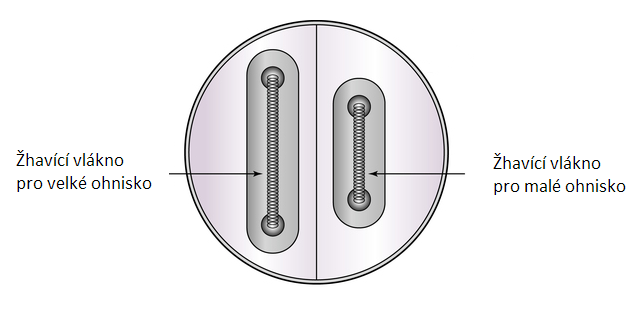
\includegraphics{cathode}
\caption{Katoda s dvěmi žhavícími vlákny. \cite{the-xray-beam}}
\label{fig:cathode}
\end{figure}
